\documentclass[]{book}
\usepackage{lmodern}
\usepackage{amssymb,amsmath}
\usepackage{ifxetex,ifluatex}
\usepackage{fixltx2e} % provides \textsubscript
\ifnum 0\ifxetex 1\fi\ifluatex 1\fi=0 % if pdftex
  \usepackage[T1]{fontenc}
  \usepackage[utf8]{inputenc}
\else % if luatex or xelatex
  \ifxetex
    \usepackage{mathspec}
  \else
    \usepackage{fontspec}
  \fi
  \defaultfontfeatures{Ligatures=TeX,Scale=MatchLowercase}
    \setmainfont[]{NanumGothic}
\fi
% use upquote if available, for straight quotes in verbatim environments
\IfFileExists{upquote.sty}{\usepackage{upquote}}{}
% use microtype if available
\IfFileExists{microtype.sty}{%
\usepackage{microtype}
\UseMicrotypeSet[protrusion]{basicmath} % disable protrusion for tt fonts
}{}
\usepackage{hyperref}
\hypersetup{unicode=true,
            pdftitle={전공의 정원관련 신경과 보고서},
            pdfauthor={중앙대학교 신경과학교실 박광열},
            pdfborder={0 0 0},
            breaklinks=true}
\urlstyle{same}  % don't use monospace font for urls
\usepackage{natbib}
\bibliographystyle{apalike}
\usepackage{color}
\usepackage{fancyvrb}
\newcommand{\VerbBar}{|}
\newcommand{\VERB}{\Verb[commandchars=\\\{\}]}
\DefineVerbatimEnvironment{Highlighting}{Verbatim}{commandchars=\\\{\}}
% Add ',fontsize=\small' for more characters per line
\usepackage{framed}
\definecolor{shadecolor}{RGB}{248,248,248}
\newenvironment{Shaded}{\begin{snugshade}}{\end{snugshade}}
\newcommand{\AlertTok}[1]{\textcolor[rgb]{0.94,0.16,0.16}{#1}}
\newcommand{\AnnotationTok}[1]{\textcolor[rgb]{0.56,0.35,0.01}{\textbf{\textit{#1}}}}
\newcommand{\AttributeTok}[1]{\textcolor[rgb]{0.77,0.63,0.00}{#1}}
\newcommand{\BaseNTok}[1]{\textcolor[rgb]{0.00,0.00,0.81}{#1}}
\newcommand{\BuiltInTok}[1]{#1}
\newcommand{\CharTok}[1]{\textcolor[rgb]{0.31,0.60,0.02}{#1}}
\newcommand{\CommentTok}[1]{\textcolor[rgb]{0.56,0.35,0.01}{\textit{#1}}}
\newcommand{\CommentVarTok}[1]{\textcolor[rgb]{0.56,0.35,0.01}{\textbf{\textit{#1}}}}
\newcommand{\ConstantTok}[1]{\textcolor[rgb]{0.00,0.00,0.00}{#1}}
\newcommand{\ControlFlowTok}[1]{\textcolor[rgb]{0.13,0.29,0.53}{\textbf{#1}}}
\newcommand{\DataTypeTok}[1]{\textcolor[rgb]{0.13,0.29,0.53}{#1}}
\newcommand{\DecValTok}[1]{\textcolor[rgb]{0.00,0.00,0.81}{#1}}
\newcommand{\DocumentationTok}[1]{\textcolor[rgb]{0.56,0.35,0.01}{\textbf{\textit{#1}}}}
\newcommand{\ErrorTok}[1]{\textcolor[rgb]{0.64,0.00,0.00}{\textbf{#1}}}
\newcommand{\ExtensionTok}[1]{#1}
\newcommand{\FloatTok}[1]{\textcolor[rgb]{0.00,0.00,0.81}{#1}}
\newcommand{\FunctionTok}[1]{\textcolor[rgb]{0.00,0.00,0.00}{#1}}
\newcommand{\ImportTok}[1]{#1}
\newcommand{\InformationTok}[1]{\textcolor[rgb]{0.56,0.35,0.01}{\textbf{\textit{#1}}}}
\newcommand{\KeywordTok}[1]{\textcolor[rgb]{0.13,0.29,0.53}{\textbf{#1}}}
\newcommand{\NormalTok}[1]{#1}
\newcommand{\OperatorTok}[1]{\textcolor[rgb]{0.81,0.36,0.00}{\textbf{#1}}}
\newcommand{\OtherTok}[1]{\textcolor[rgb]{0.56,0.35,0.01}{#1}}
\newcommand{\PreprocessorTok}[1]{\textcolor[rgb]{0.56,0.35,0.01}{\textit{#1}}}
\newcommand{\RegionMarkerTok}[1]{#1}
\newcommand{\SpecialCharTok}[1]{\textcolor[rgb]{0.00,0.00,0.00}{#1}}
\newcommand{\SpecialStringTok}[1]{\textcolor[rgb]{0.31,0.60,0.02}{#1}}
\newcommand{\StringTok}[1]{\textcolor[rgb]{0.31,0.60,0.02}{#1}}
\newcommand{\VariableTok}[1]{\textcolor[rgb]{0.00,0.00,0.00}{#1}}
\newcommand{\VerbatimStringTok}[1]{\textcolor[rgb]{0.31,0.60,0.02}{#1}}
\newcommand{\WarningTok}[1]{\textcolor[rgb]{0.56,0.35,0.01}{\textbf{\textit{#1}}}}
\usepackage{longtable,booktabs}
\usepackage{graphicx,grffile}
\makeatletter
\def\maxwidth{\ifdim\Gin@nat@width>\linewidth\linewidth\else\Gin@nat@width\fi}
\def\maxheight{\ifdim\Gin@nat@height>\textheight\textheight\else\Gin@nat@height\fi}
\makeatother
% Scale images if necessary, so that they will not overflow the page
% margins by default, and it is still possible to overwrite the defaults
% using explicit options in \includegraphics[width, height, ...]{}
\setkeys{Gin}{width=\maxwidth,height=\maxheight,keepaspectratio}
\IfFileExists{parskip.sty}{%
\usepackage{parskip}
}{% else
\setlength{\parindent}{0pt}
\setlength{\parskip}{6pt plus 2pt minus 1pt}
}
\setlength{\emergencystretch}{3em}  % prevent overfull lines
\providecommand{\tightlist}{%
  \setlength{\itemsep}{0pt}\setlength{\parskip}{0pt}}
\setcounter{secnumdepth}{5}
% Redefines (sub)paragraphs to behave more like sections
\ifx\paragraph\undefined\else
\let\oldparagraph\paragraph
\renewcommand{\paragraph}[1]{\oldparagraph{#1}\mbox{}}
\fi
\ifx\subparagraph\undefined\else
\let\oldsubparagraph\subparagraph
\renewcommand{\subparagraph}[1]{\oldsubparagraph{#1}\mbox{}}
\fi

%%% Use protect on footnotes to avoid problems with footnotes in titles
\let\rmarkdownfootnote\footnote%
\def\footnote{\protect\rmarkdownfootnote}

%%% Change title format to be more compact
\usepackage{titling}

% Create subtitle command for use in maketitle
\providecommand{\subtitle}[1]{
  \posttitle{
    \begin{center}\large#1\end{center}
    }
}

\setlength{\droptitle}{-2em}

  \title{전공의 정원관련 신경과 보고서}
    \pretitle{\vspace{\droptitle}\centering\huge}
  \posttitle{\par}
    \author{중앙대학교 신경과학교실 박광열}
    \preauthor{\centering\large\emph}
  \postauthor{\par}
      \predate{\centering\large\emph}
  \postdate{\par}
    \date{2019-10-01}

\usepackage{booktabs}

\begin{document}
\maketitle

{
\setcounter{tocdepth}{1}
\tableofcontents
}
\hypertarget{things-to-be-done}{%
\chapter*{Things to be done}\label{things-to-be-done}}
\addcontentsline{toc}{chapter}{Things to be done}

\begin{enumerate}
\def\labelenumi{\arabic{enumi}.}
\tightlist
\item
  KPS연구를 중심으로 기존 추계연구 critical review
\item
  해외 연구 현황 추가
\end{enumerate}

\hypertarget{DemandSupplyNeurologist}{%
\chapter{신경과 전문의 수급현황}\label{DemandSupplyNeurologist}}

\hypertarget{section}{%
\section{인구 10만명당 신경과 전문의 수}\label{section}}

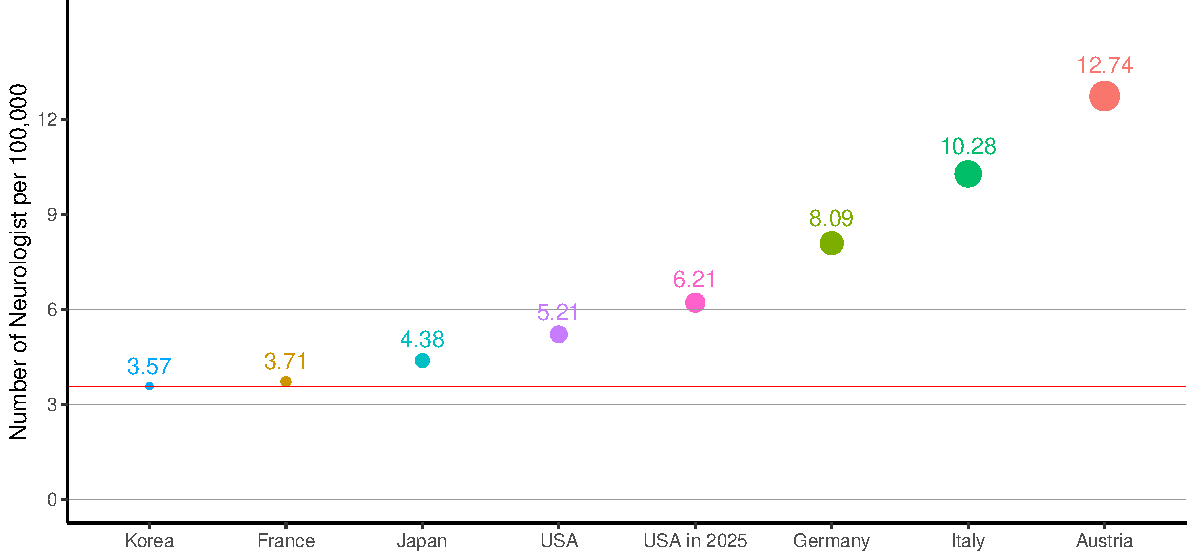
\includegraphics{Neurology_Report_Resident_TO_files/figure-latex/unnamed-chunk-3-1.pdf}

• 인구 10만명당 신경과 전문의의 숫자는 한국이 3.57명 (2018년기준)으로 네덜란드, 일본, 헝가리, 스위스, 칠레 등에 비해 적음.

• 통계청 자료에 의한 2018년 인구는 51,014,947명으로, 인구 10만명당 신경과 전문의 수가 네덜란드 수준인 6명이 되려면 3060명이 필요함 (2018년 전문의 수가1845명이므로 부족분은 1215명).

• 미국의 경우 2012년 기준 인구 10만명당 신경과 전문의는 5.21명이며 2025년에는 6.21명이 필요할 것으로 예상되고 있음.

\hypertarget{section-1}{%
\section{한국의 신경과 전문의 연령별 분포 (2018.4기준)}\label{section-1}}

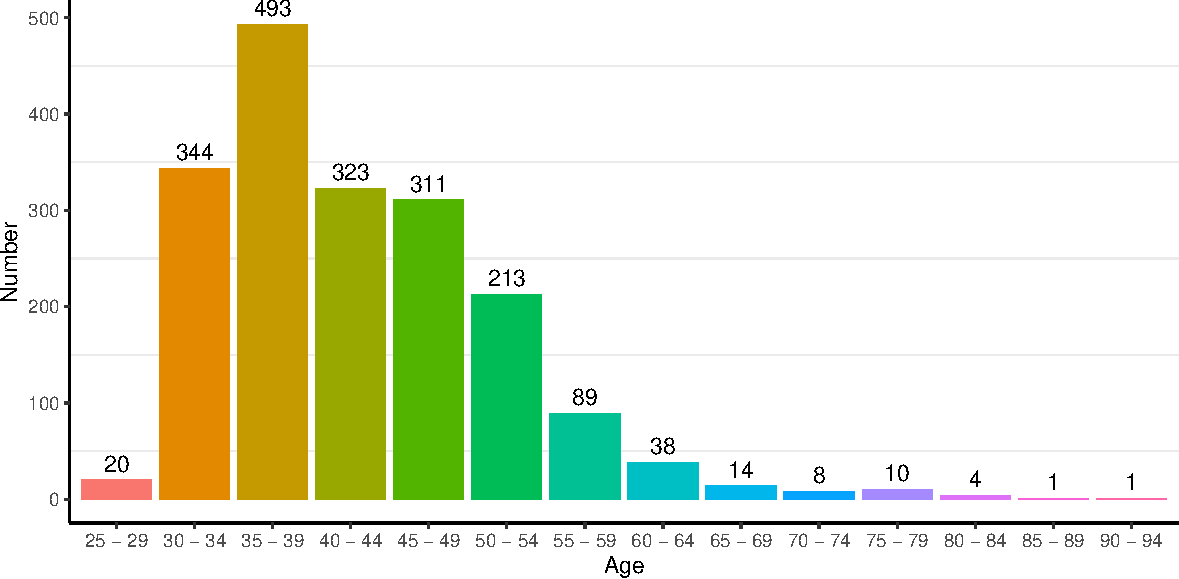
\includegraphics{Neurology_Report_Resident_TO_files/figure-latex/unnamed-chunk-5-1.pdf}

\hypertarget{section-2}{%
\chapter{국내외 선행연구 고찰}\label{section-2}}

\hypertarget{section-3}{%
\section{2017.9 전공의 정원정책 수립을 위한 전문의 인력 수요 추계 연구 보고서}\label{section-3}}

\hypertarget{section-4}{%
\subsection{서론}\label{section-4}}

\begin{itemize}
\item
  의료인력의 쏠림: 지역별, 전문과목별
\item
  수급의 불균형: 의료인력의 고령화, 인구의 변화, 수요의 증가, 지역적 편재, (전문과목별 편재)
\item
  추계접근방법: 전통적 접근법과 통합적 접근법
\item
  전공의를 근로자로 인식하는 잘못된 인식. 수련병원의 인력수요에 대응하는 정원정책이 아닌 고령화, 만성질환증가 등에 대응하는 추계가 필요함

  \begin{itemize}
  \tightlist
  \item
    그러나, 현실적으로는 전공의가 의료의 상당부분을 담당하고 있음. 또한, 전공의가 없을 경우, 대부분의 수련병원에서 의료공백이 발생할것이 명백함. 전공의의 공백을 채울 전문의가 아직 없음. 따라서, 현실을 고려하지 않은 발상임.
  \item
    또한, 이런 생각이라면, 공급추계를 할 때, 전공의를 의료인력에서 제외해야 함 (공급추계에서 제외)
  \end{itemize}
\item
  전문과목별 의료 이용량및 질병양상 예측을 통해 의료이용추계를 하고자 함.
\item
  공급: 유입유출법, 수요: 전문의 1일 생산성과 환자 의료 이용율을 이용한 의료수요 계측법

  \begin{itemize}
  \tightlist
  \item
    신경과와 같이 유출이 적은 경우에는 유입유출법을 적용할 수 없음.
  \item
    특히 전문의의 노화에 대한 고려가 있어야 함.
  \end{itemize}
\item
  전문의가 해당 전문과목의 전문의로 기능하고 있는 경우: 18 \%
\item
  전문과목별 쏠림현상의 개선을 위해 진행.

  \begin{itemize}
  \item
    정원이 줄어들면서 오히려 지원이 감소하는 경우도 있음.
  \item
    한국은 의료이용시의 장애가 낮은 편인데 OECD와 비교하는 것이 맞을지?
  \item
    공급모형에서는 전공의 충원률 또는 지원률이 같이 고려되어야 함.
  \item
    실제 일하는 인력에 대한 조사가 정기적으로 필요함.
  \item
    수요추계모형에서는 인구학적인 요인과 더불어 보험적용기준의 변화에 따른 변화 (MRI의 보험적용등)가 같이 고려되어야 함.
  \item
    앞으로 의료인력 추계 모형연구는 reproducibility가 담보될 수 있도록 raw data를 공개해야 한다.
  \end{itemize}
\end{itemize}

\hypertarget{section-5}{%
\subsection{전문의 수요 추계}\label{section-5}}

\begin{itemize}
\tightlist
\item
  국내 한국보건사회연구원 오영호(2011, 2014)의 연구와, 정형선(2011)의 연구 및 미국 Bureau of Health Workforce 모형을 참조하여 개발
\end{itemize}

\hypertarget{section-6}{%
\subsubsection{공급추정: 전문의사수}\label{section-6}}

\begin{verbatim}
- 전공의를 고려해야 함
- 현재 시스템에서는 전공의인력이 의료공급의 상당부분을 차지하고 있는데, 전공의를 감소시킨다면 그만큼 전문의가 더 필요함에도 이에 대한 고려가 없음. (전공의가 없으면 전문의의 생산성이 떨어지기 때문)
\end{verbatim}

\begin{itemize}
\item
  의사에 대한 공급량은 실제 활동하고 있는 의사 수에 의해 측정하되, 심사평가 원에서 제공된 자료 이용
\item
  의사의 연간 근무일수: 365 - (법정공휴일 66일 + 주5일 51일 + 학회 10일)

  \begin{itemize}
  \tightlist
  \item
    1년중 평일\textgreater{} 249일, 휴일\textgreater{} 116일. \url{https://zetawiki.com/wiki/연간_공휴일_수,_영업일_수,_근무일_수}
  \item
    연차 휴가: 간단한 근속년수에 따른 연차가산일 수식 = (근속년수- 1년)/2 (나머지 버림) \url{https://help.jobis.co/hc/ko/articles/115003127813--연차-근로기간에-따른-연차휴가}
  \item
    출산휴가(90일), 육아휴직 \url{https://help.jobis.co/hc/ko/articles/360001561894--노무-출산휴가-육아휴직-알아보기-}
  \end{itemize}
\end{itemize}

\hypertarget{section-7}{%
\subsubsection{전제조건}\label{section-7}}

\begin{itemize}
\item
  현재의 급여 및 연령 구조 동일

  \begin{itemize}
  \tightlist
  \item
    연령구조가 동일하다는 것은 신생과의 경우에는 맞지 않음.
  \end{itemize}
\item
  전체 이용량에서 외래에 대비한 입원의 비중이 변화하지 않고 현재 상태 유지함.
\item
  의사 1인당 생산성의 변화는 없음

  \begin{itemize}
  \tightlist
  \item
    전공의가 없어지면서 1인당 생산성을 떨어짐.
  \item
    전공의 특별법의 영향.
  \end{itemize}
\item
  건강보험과 의료급여 포함

  \begin{itemize}
  \tightlist
  \item
    비급여에 대한 고민 ?
  \end{itemize}
\end{itemize}

\hypertarget{section-8}{%
\subsubsection{수요추정}\label{section-8}}

\begin{itemize}
\item
  수요 추정을 위한 의료이용량은 2012-2016년 건강보험, 의료급여 및 보훈 병원 의 의원급 병원급 진료 과목별 심사실적을 사용
\item
  2018-2022년의 의료 공급과 수요를 계산하기 위해서, 공급은 최근 5년간의 평 균 증가율인 3.7\% 그리고 수요도 최근 5년간의 평균 증가율인 2.7\%를 적용함
\item
  이 평균 증가율은 정형선(2011)의 자료와 차이를 보이는데(수요 평균 증가율 6\textasciitilde7\%). 이는 최근의 경기 불황으로 의료 수요의 증가폭이 줄어든 것이 반영된 것임.

  \begin{itemize}
  \tightlist
  \item
    2015년 MERS사태가 고려되지 않음.
  \item
    2015년 IA thrombectomy에 대한 연구 다수 발표. 이후 혈전제거술의 time window가 늘어남.
  \end{itemize}
\item
  환자 1인당 평균진료시간: 7.9분 (신경과), 8.1분 (일반외과),
\end{itemize}

\hypertarget{kps}{%
\section{5개과 설문분석 결과와 KPS}\label{kps}}

NU: 238, KPS 193

\hypertarget{section-9}{%
\chapter{전문의 수급에 영향을 줄 만한 정책적 이슈}\label{section-9}}

1-2 page

\begin{itemize}
\item
  (이 부분은 해당 전문과별로 특별한 이슈가 있는 경우에만 적용하는 것이 좋을 듯 합니다만, 전문과목과 무관하게 의료계의 정책적인 변화가 수급 전반에 걸쳐 큰 영향을 준다고 판단하신다면, 전문과목별 작성 내용에서 다루지 않고 전체 내용을 다루는 챕터에서 별도로 다루시는 게 좋을 듯 합니다.)
\item
  예를 들어, 문재인 케어와 같은 정책변화는 전 의료계에 영향을 줄 수 있는 요인이고 그 내부에 과목별 특이적인 사항(ex. 특정 시술 또는 처방에 대한 보장성 강화로 급여 확대)이 있다면, 이는 어떤 챕터에서 다룰 지 내부 논의가 필요할 것 같습니다.
\end{itemize}

\hypertarget{section-10}{%
\chapter{전문의 수급 추계에 관한 문제제기}\label{section-10}}

(2, 3번 내용을 토대로) 전문의 수급 추계에 관한 문제제기 (1\textasciitilde2page)

(2, 3번의 내용을 모두 전문과목별 작성 챕터에서 다루시게 될 경우 둘의 순서는 바꾸어도 무방할 듯 함.)

-국내외 선행연구 고찰 및 정책적 이슈로 인한 변화(영향)을 통해 현재 전문의 수급 현황, 적정 전문의 수 추계 과정 및 방법, 관계부처와 관련된 특이사항 등을 포괄하여 문제점으로 제시될 수 있는 다양한 내용을 도출. 국외와 비교하는 내용도 좋음.

-이 챕터에서는 특히나 소제목으로 범주화하여 내용을 기술하는 것이 중요할 것임.
-(그러나, 만약 5개 전문과목별로 문제제기 내용이 대동소이하다면, 이 부분 역시 특정 전문과목에 제한하지 말고 전체 전문과목에 대한 소결 정도로 도출하면 좋을 듯 합니다.)

\hypertarget{example-one}{%
\section{Example one}\label{example-one}}

\hypertarget{example-two}{%
\section{Example two}\label{example-two}}

\hypertarget{section-11}{%
\chapter{소결론}\label{section-11}}

\begin{itemize}
\tightlist
\item
  (해당과) 전문과목에 대해 핵심적으로 도출할만한 내용을 소결로 작성해 주시면, 과별 내용을 간단명료하게 확인할 수 있을 뿐 아니라, 이후 전체 보고서의 결론에 소결의 내용을 모아 작성하는 데 큰 도움이 될 듯 합니다.
\end{itemize}

\hypertarget{survey}{%
\chapter{Survey}\label{survey}}

\hypertarget{section-12}{%
\section{전반적인 요약}\label{section-12}}

The number of total respondent: 2497

The number of reliable respondent: 1769

\hypertarget{section-13}{%
\subsection{전공별 참여 인원}\label{section-13}}

Specialty

CS : 64

GS :341

NU :238

PED:572

PSY:554

\hypertarget{section-14}{%
\subsection{신경과 의사중 급성 뇌경색 치료에 참여하는 인원}\label{section-14}}

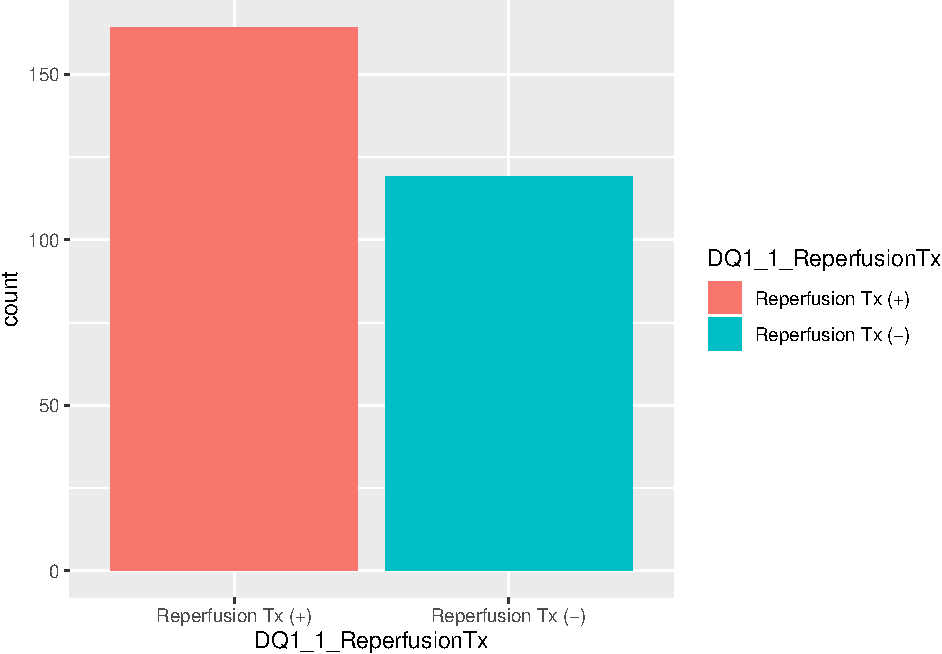
\includegraphics{Neurology_Report_Resident_TO_files/figure-latex/unnamed-chunk-11-1.pdf}

\begin{itemize}
\tightlist
\item
  신경과 의사중 57.14\%가 급성 뇌경색 치료에 참여하고 있음.
\end{itemize}

\hypertarget{section-15}{%
\subsection{전공의 참여자수}\label{section-15}}

\begin{verbatim}
##    
##     CS GS NU PED PSY
##   1  0  0  0  10  10
##   2  0  0  4   8  11
##   3  0  0 11  10  10
##   4  1  0  9  14  15
\end{verbatim}

\begin{itemize}
\tightlist
\item
  전공의의 숫자가 적어서 전공의의 상황을 알기 어려움
\end{itemize}

\hypertarget{a.-}{%
\section{A. 근무시간}\label{a.-}}

\hypertarget{section-16}{%
\subsection{과별 주중 근무시간 (평균, 최대, 최소, 표준편차)}\label{section-16}}

Specialty

Mean work hour

Max

Min

Standard Deviaiton

CS

10.88

18

6

2.40

GS

10.38

24

4

2.67

NU

10.71

18

5

2.34

PED

8.89

24

2

2.19

PSY

8.51

18

3

1.57

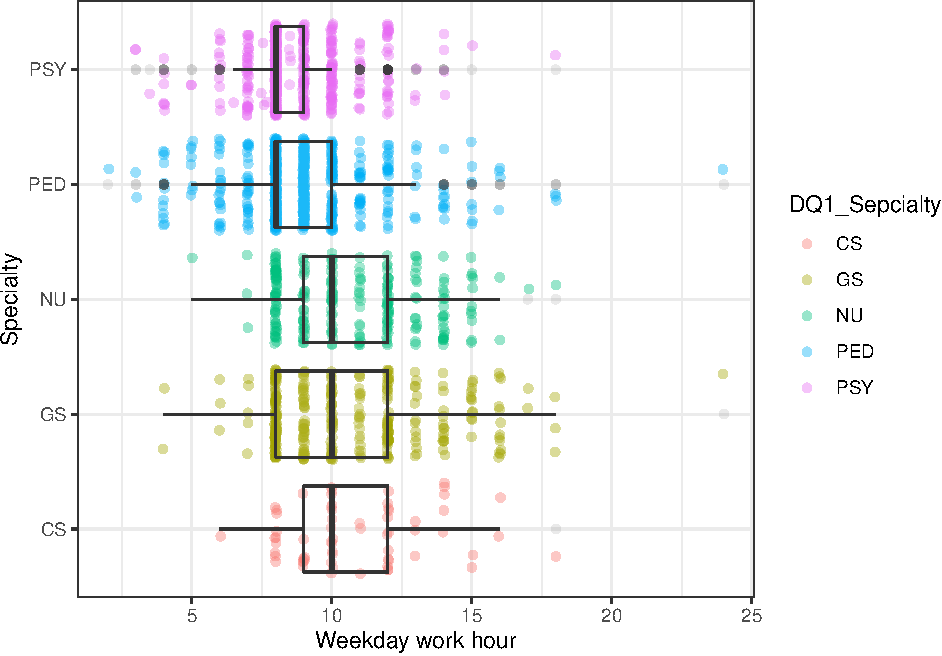
\includegraphics{Neurology_Report_Resident_TO_files/figure-latex/unnamed-chunk-14-1.pdf}

\begin{itemize}
\tightlist
\item
  평균적으로 흉부외과, 일반외과, 신경과의 평균 주중 근무시간이 길다.
\end{itemize}

ReperfusionTx

Mean work hour

Max

Min

Standard Deviaiton

Reperfusion Tx (-)

10.15

15

5

2.33

Reperfusion Tx (+)

11.13

18

8

2.26

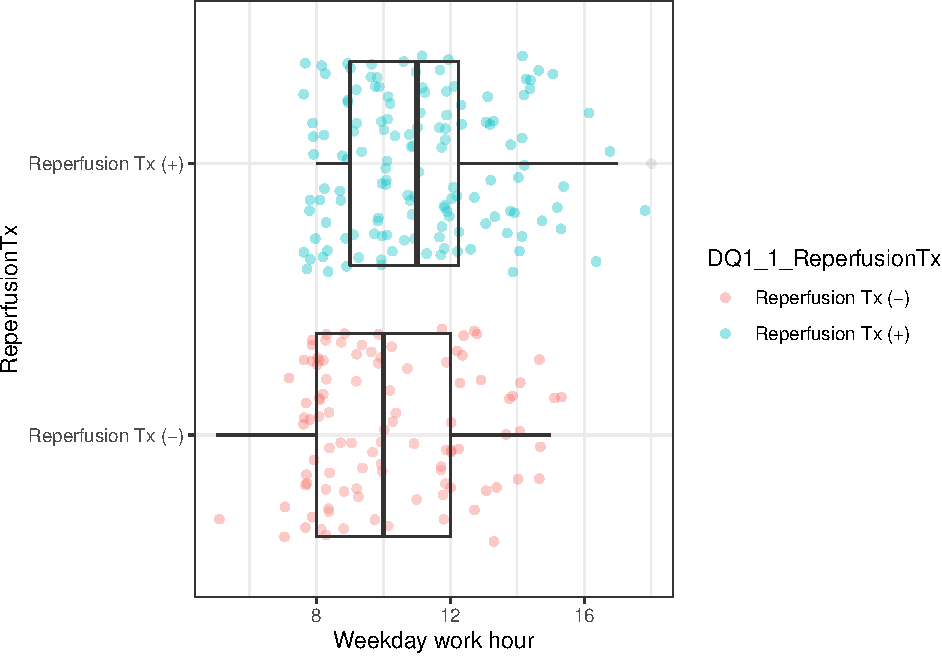
\includegraphics{Neurology_Report_Resident_TO_files/figure-latex/unnamed-chunk-16-1.pdf}

\begin{itemize}
\item
  또한, 신경과 의사중에서도 급성기 뇌경색 치료를 담당하는 인력의 평균 근무시간을 더 길다.
\item
  위의 결과를 보면 과별로도 근무시간이 차이가 나며, 같은 과 내에서도 응급질환의 진료여부에 따라 근무 부담에 차이가 난다.
\end{itemize}

\begin{Shaded}
\begin{Highlighting}[]
\NormalTok{db }\OperatorTok\StringTok{ }\KeywordTok{group_by}\NormalTok{(DQ1_Sepcialty) }\OperatorTok
\StringTok{  }\KeywordTok{summarise}\NormalTok{(}\DataTypeTok{meanworkhour =} \KeywordTok{mean}\NormalTok{(A1_}\DecValTok{2}\NormalTok{_worktime_saturday, }\DataTypeTok{na.rm =}\NormalTok{ T),}
            \DataTypeTok{maxworkhour =} \KeywordTok{max}\NormalTok{(A1_}\DecValTok{2}\NormalTok{_worktime_saturday, }\DataTypeTok{na.rm =}\NormalTok{ T),}
            \DataTypeTok{minworkhour =} \KeywordTok{min}\NormalTok{(A1_}\DecValTok{2}\NormalTok{_worktime_saturday, }\DataTypeTok{na.rm =}\NormalTok{ T))}
\end{Highlighting}
\end{Shaded}

\begin{verbatim}
## # A tibble: 5 x 4
##   DQ1_Sepcialty meanworkhour maxworkhour minworkhour
##   <fct>                <dbl>       <dbl>       <dbl>
## 1 CS                    4.94          24           1
## 2 GS                    4.45          24           1
## 3 NU                    4.86          24           1
## 4 PED                   5.15          24           1
## 5 PSY                   4.62          24           1
\end{verbatim}

\begin{Shaded}
\begin{Highlighting}[]
\KeywordTok{ggplot}\NormalTok{(db, }\KeywordTok{aes}\NormalTok{(}\DataTypeTok{x =}\NormalTok{ DQ1_Sepcialty, }\DataTypeTok{y =}\NormalTok{ A1_}\DecValTok{2}\NormalTok{_worktime_saturday)) }\OperatorTok{+}
\StringTok{  }\KeywordTok{geom_boxplot}\NormalTok{(}\KeywordTok{aes}\NormalTok{(}\DataTypeTok{fill =}\NormalTok{ DQ1_Sepcialty), }\DataTypeTok{alpha =} \FloatTok{0.1}\NormalTok{) }\OperatorTok{+}\StringTok{ }
\StringTok{  }\KeywordTok{geom_jitter}\NormalTok{(}\KeywordTok{aes}\NormalTok{(}\DataTypeTok{color =}\NormalTok{ DQ1_Sepcialty, }\DataTypeTok{alpha =} \FloatTok{0.1}\NormalTok{)) }\OperatorTok{+}
\StringTok{  }\KeywordTok{scale_x_discrete}\NormalTok{(}\DataTypeTok{limits =} \KeywordTok{c}\NormalTok{(}\StringTok{"PED"}\NormalTok{, }\StringTok{"GS"}\NormalTok{, }\StringTok{"PSY"}\NormalTok{, }\StringTok{"CS"}\NormalTok{, }\StringTok{"NU"}\NormalTok{, }\StringTok{"Multi"}\NormalTok{))}
\end{Highlighting}
\end{Shaded}

\begin{verbatim}
## Warning: Removed 429 rows containing non-finite values (stat_boxplot).
\end{verbatim}

\begin{verbatim}
## Warning: Removed 429 rows containing missing values (geom_point).
\end{verbatim}

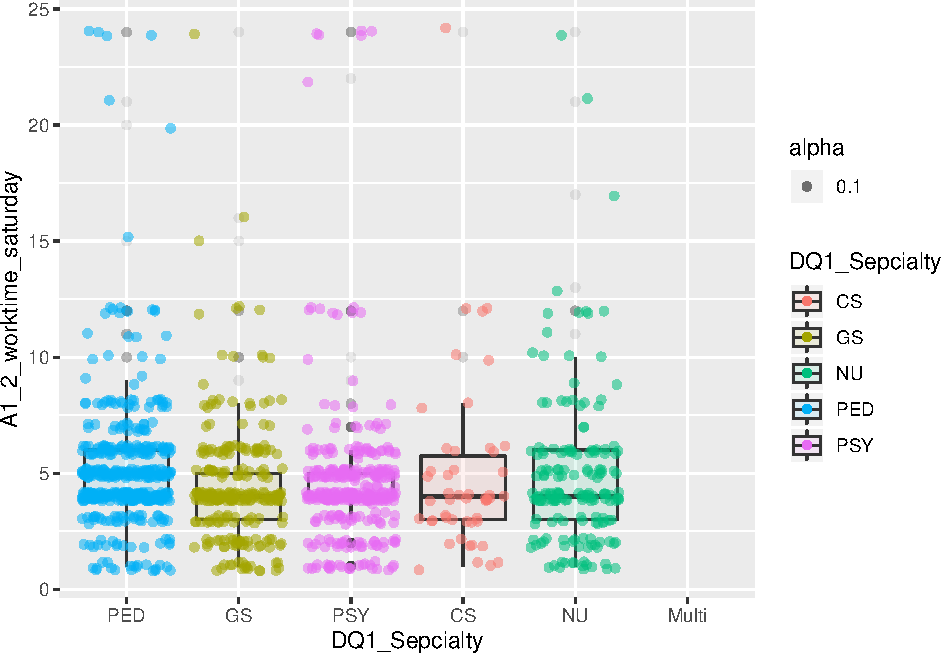
\includegraphics{Neurology_Report_Resident_TO_files/figure-latex/unnamed-chunk-17-1.pdf}

\begin{Shaded}
\begin{Highlighting}[]
\NormalTok{db }\OperatorTok\StringTok{ }\KeywordTok{group_by}\NormalTok{(DQ1_Sepcialty) }\OperatorTok
\StringTok{  }\KeywordTok{summarise}\NormalTok{(}\DataTypeTok{meanworkhour =} \KeywordTok{mean}\NormalTok{(A1_}\DecValTok{3}\NormalTok{_worktime_sunday, }\DataTypeTok{na.rm =}\NormalTok{ T),}
            \DataTypeTok{maxworkhour =} \KeywordTok{max}\NormalTok{(A1_}\DecValTok{3}\NormalTok{_worktime_sunday, }\DataTypeTok{na.rm =}\NormalTok{ T),}
            \DataTypeTok{minworkhour =} \KeywordTok{min}\NormalTok{(A1_}\DecValTok{3}\NormalTok{_worktime_sunday, }\DataTypeTok{na.rm =}\NormalTok{ T))}
\end{Highlighting}
\end{Shaded}

\begin{verbatim}
## # A tibble: 5 x 4
##   DQ1_Sepcialty meanworkhour maxworkhour minworkhour
##   <fct>                <dbl>       <dbl>       <dbl>
## 1 CS                    5.67          24           1
## 2 GS                    4.38          24           1
## 3 NU                    5.52          24           1
## 4 PED                   5.93          24           1
## 5 PSY                   7             24           1
\end{verbatim}

\begin{Shaded}
\begin{Highlighting}[]
\KeywordTok{ggplot}\NormalTok{(db, }\KeywordTok{aes}\NormalTok{(}\DataTypeTok{x =}\NormalTok{ DQ1_Sepcialty, }\DataTypeTok{y =}\NormalTok{ A1_}\DecValTok{3}\NormalTok{_worktime_sunday)) }\OperatorTok{+}
\StringTok{  }\KeywordTok{geom_boxplot}\NormalTok{(}\KeywordTok{aes}\NormalTok{(}\DataTypeTok{fill =}\NormalTok{ DQ1_Sepcialty), }\DataTypeTok{alpha =} \FloatTok{0.1}\NormalTok{) }\OperatorTok{+}\StringTok{ }
\StringTok{  }\KeywordTok{geom_jitter}\NormalTok{(}\KeywordTok{aes}\NormalTok{(}\DataTypeTok{color =}\NormalTok{ DQ1_Sepcialty, }\DataTypeTok{alpha =} \FloatTok{0.1}\NormalTok{)) }\OperatorTok{+}
\StringTok{  }\KeywordTok{scale_x_discrete}\NormalTok{(}\DataTypeTok{limits =} \KeywordTok{c}\NormalTok{(}\StringTok{"PED"}\NormalTok{, }\StringTok{"GS"}\NormalTok{, }\StringTok{"PSY"}\NormalTok{, }\StringTok{"CS"}\NormalTok{, }\StringTok{"NU"}\NormalTok{, }\StringTok{"Multi"}\NormalTok{))}
\end{Highlighting}
\end{Shaded}

\begin{verbatim}
## Warning: Removed 1280 rows containing non-finite values (stat_boxplot).
\end{verbatim}

\begin{verbatim}
## Warning: Removed 1280 rows containing missing values (geom_point).
\end{verbatim}

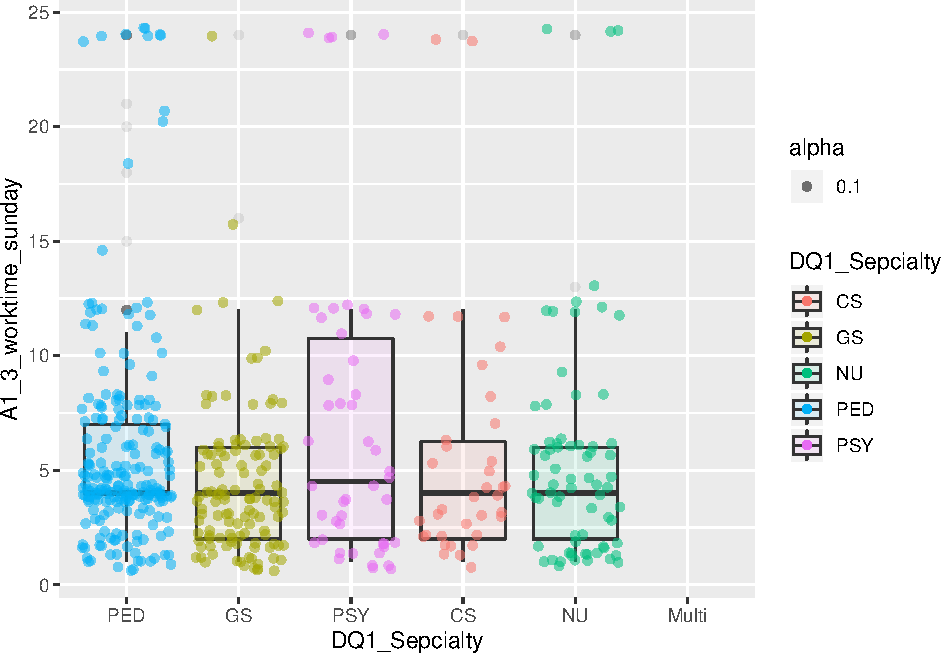
\includegraphics{Neurology_Report_Resident_TO_files/figure-latex/unnamed-chunk-17-2.pdf}

\begin{Shaded}
\begin{Highlighting}[]
\NormalTok{db }\OperatorTok\StringTok{ }\KeywordTok{group_by}\NormalTok{(DQ1_Sepcialty) }\OperatorTok
\StringTok{  }\KeywordTok{summarise}\NormalTok{(}\DataTypeTok{meanworkhour =} \KeywordTok{mean}\NormalTok{(A2_meanworkhourperweek, }\DataTypeTok{na.rm =}\NormalTok{ T),}
            \DataTypeTok{maxworkhour =} \KeywordTok{max}\NormalTok{(A2_meanworkhourperweek, }\DataTypeTok{na.rm =}\NormalTok{ T),}
            \DataTypeTok{minworkhour =} \KeywordTok{min}\NormalTok{(A2_meanworkhourperweek, }\DataTypeTok{na.rm =}\NormalTok{ T))}
\end{Highlighting}
\end{Shaded}

\begin{verbatim}
## # A tibble: 5 x 4
##   DQ1_Sepcialty meanworkhour maxworkhour minworkhour
##   <fct>                <dbl>       <dbl>       <dbl>
## 1 CS                    63.7         110           8
## 2 GS                    56.0         120           6
## 3 NU                    58.5         114           7
## 4 PED                   48.4         120           7
## 5 PSY                   44.4         100           5
\end{verbatim}

\begin{Shaded}
\begin{Highlighting}[]
\KeywordTok{ggplot}\NormalTok{(db, }\KeywordTok{aes}\NormalTok{(}\DataTypeTok{x =}\NormalTok{ DQ1_Sepcialty, }\DataTypeTok{y =}\NormalTok{ A2_meanworkhourperweek)) }\OperatorTok{+}
\StringTok{  }\KeywordTok{geom_boxplot}\NormalTok{(}\KeywordTok{aes}\NormalTok{(}\DataTypeTok{fill =}\NormalTok{ DQ1_Sepcialty), }\DataTypeTok{alpha =} \FloatTok{0.1}\NormalTok{) }\OperatorTok{+}\StringTok{ }
\StringTok{  }\KeywordTok{geom_jitter}\NormalTok{(}\KeywordTok{aes}\NormalTok{(}\DataTypeTok{color =}\NormalTok{ DQ1_Sepcialty, }\DataTypeTok{alpha =} \FloatTok{0.1}\NormalTok{)) }\OperatorTok{+}
\StringTok{  }\KeywordTok{scale_x_discrete}\NormalTok{(}\DataTypeTok{limits =} \KeywordTok{c}\NormalTok{(}\StringTok{"PED"}\NormalTok{, }\StringTok{"GS"}\NormalTok{, }\StringTok{"PSY"}\NormalTok{, }\StringTok{"CS"}\NormalTok{, }\StringTok{"NU"}\NormalTok{, }\StringTok{"Multi"}\NormalTok{))}
\end{Highlighting}
\end{Shaded}

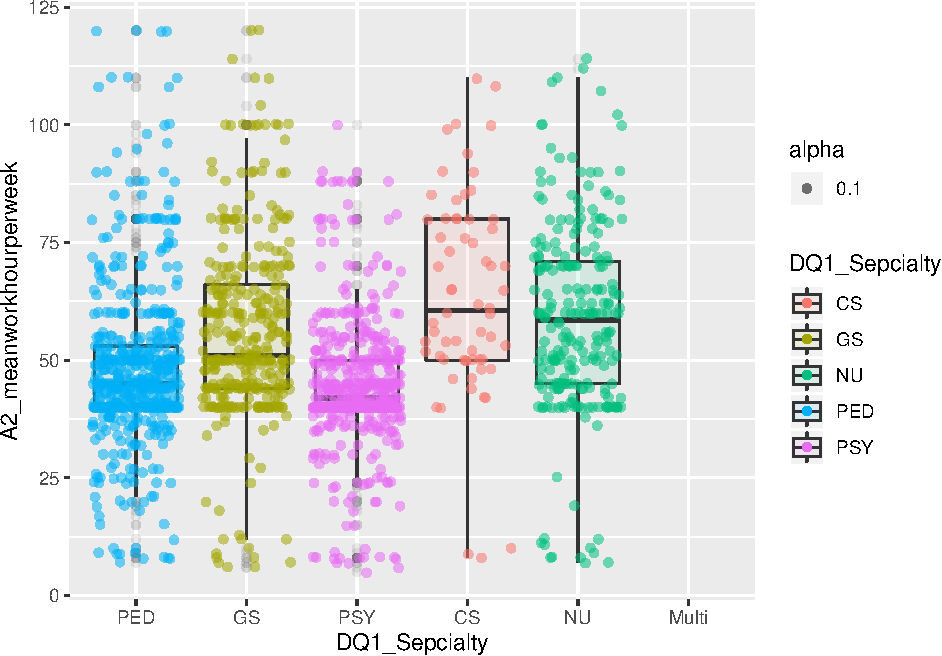
\includegraphics{Neurology_Report_Resident_TO_files/figure-latex/unnamed-chunk-17-3.pdf}

\bibliography{book.bib,packages.bib}


\end{document}
